\question \textbf{Maximum parsimony}

The maximum parsimony uses column-wise operations of union and intersection. The number of union operations is counted to find the tree that minimizes the evolutionary changes. \\

\begin{figure}[H]
      \centering
      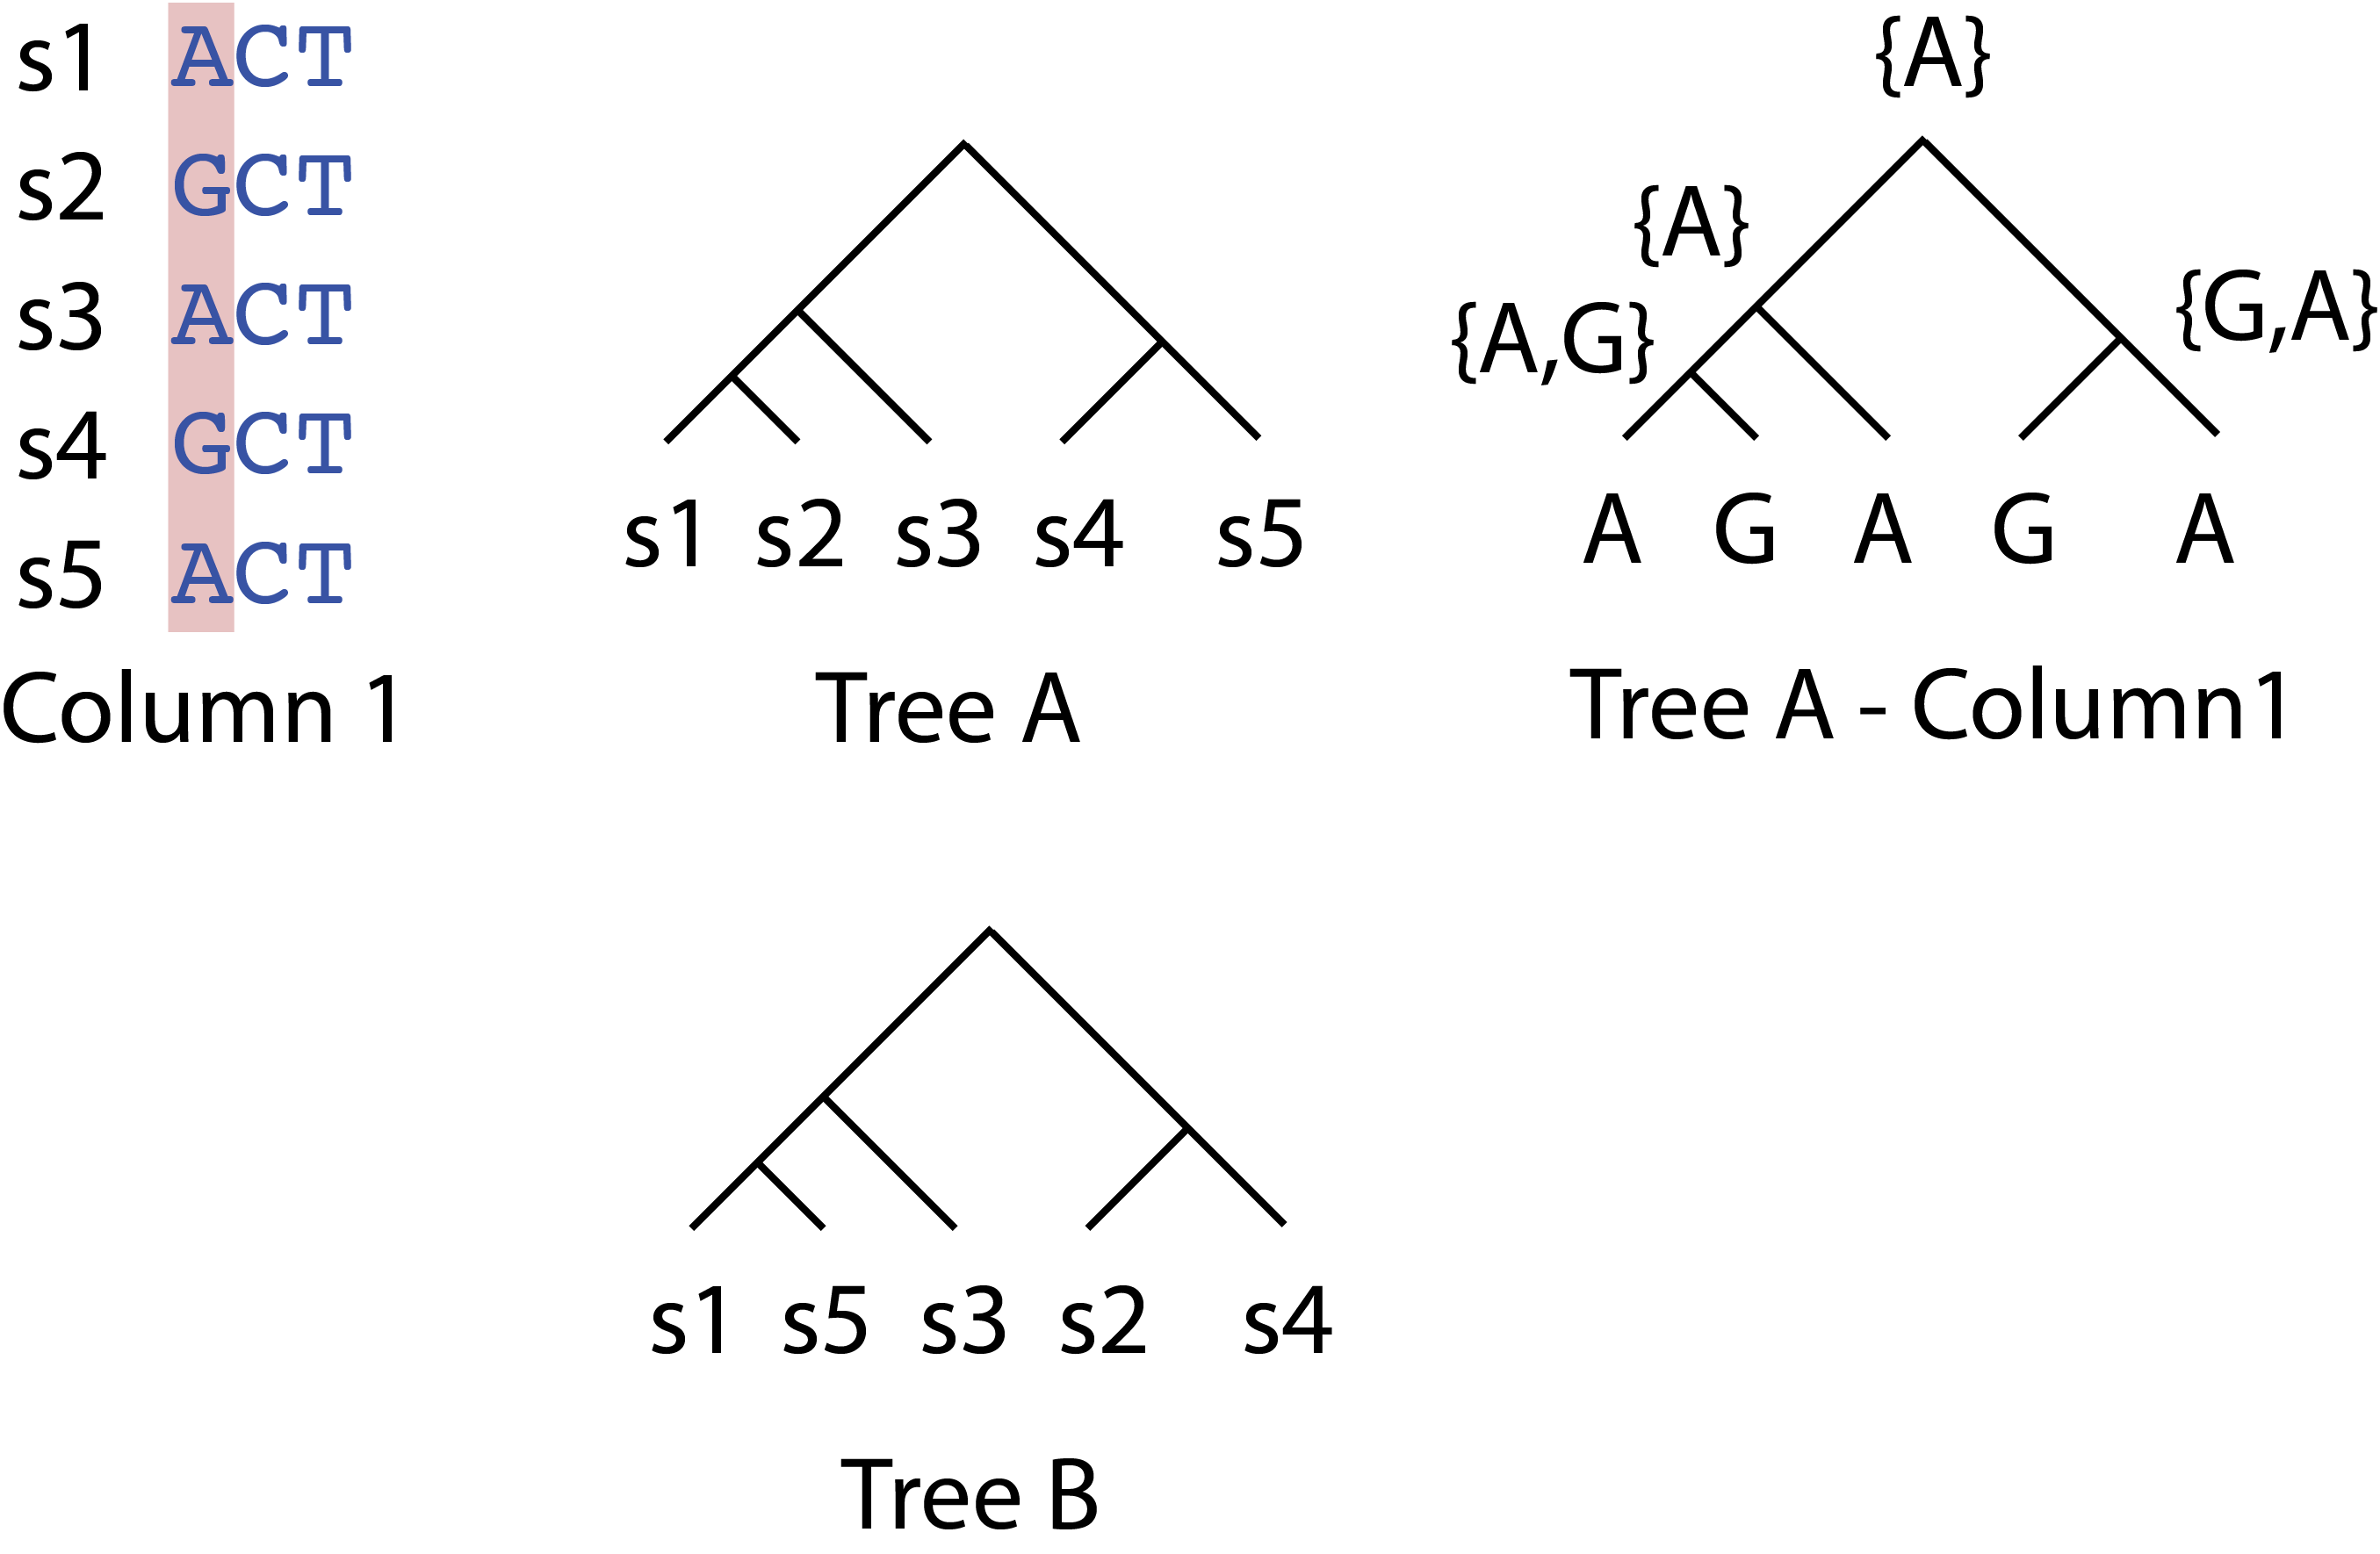
\includegraphics[width=0.5 \textwidth]{fig09/maximum_parsimony_tree_a.png}
\end{figure}

Use the first column of the MSA and also Tree A and B to answer the following questions.

\vspace{0.1 in}

\begin{parts}

%% (a)
  \part How many union operations are necessary to estimate the labels of the root and the internal nodes of Tree A?

\begin{solution}[0.35 in]
2
\end{solution}

%% (b)
  \part Estimate the labels of the root and the internal nodes of Tree B.
  
\begin{figure}[H]
      \centering
      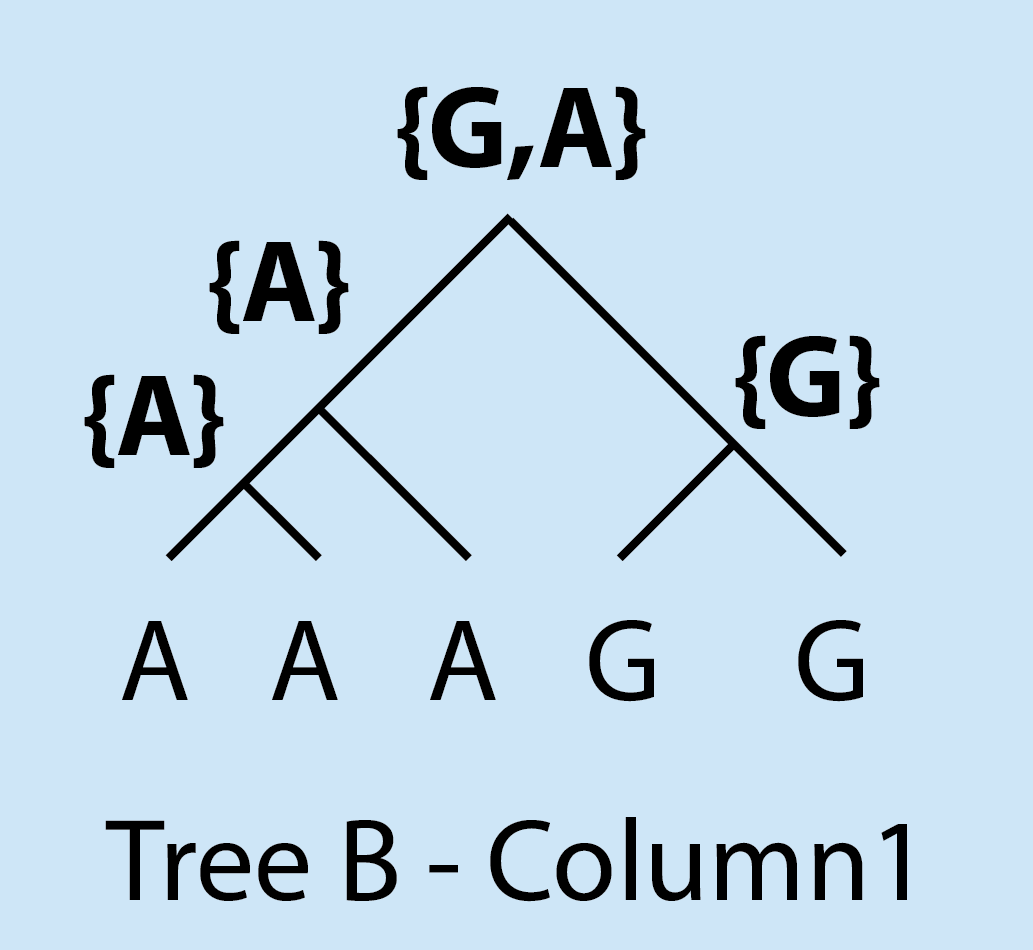
\includegraphics[width=0.2 \textwidth]{fig09/maximum_parsimony_tree_b_solution.png}
\end{figure}

%% (c)
  \part How many union operations are necessary to estimate the root and the internal nodes of Tree B?
  
\begin{solution}[0.35 in]
1
\end{solution}

%% (d)
  \part  Which tree, Tree A or B, indicates less evolutionary changes when only the first column is considered?
  
\begin{solution}[0.35 in]
Tree B
\end{solution}

  
\end{parts}

